\documentclass{beamer}
\setbeamertemplate{navigation symbols}{}
% \usetheme{Bergen}
\usecolortheme{beaver}
\usepackage[T1]{fontenc}
\usepackage[utf8]{inputenc}
\usepackage{fontawesome}
\beamersetuncovermixins{\opaqueness<1>{25}}{\opaqueness<2->{15}}
\setbeamerfont{alerted text}{series=\LARGE\bfseries}
\setbeamertemplate{frametitle}[default][center]
\newcommand{\btVFill}{\vskip0pt plus 1filll}
\setbeamersize{text margin left=3mm,text margin right=3mm}
\newcommand{\ra}{$\rightarrow$}
\newcommand{\biz}{\textcolor{magenta}{\faBriefcase}}

\begin{document}

\begin{frame}[t]{First-principles modelling of 2D semiconductors}

I use our best understanding of electrons, protons, and how they glue together
(quantum mechanics) to try to \textcolor{magenta}{predict} things.
\vspace{.4cm}

\begin{minipage}[t]{0.33\textwidth}

\begin{center}
{\bf What?}
\begin{itemize}
  \item Energy gaps
  \item Exciton levels
\end{itemize}

\begin{figure}[h]
  \centering
  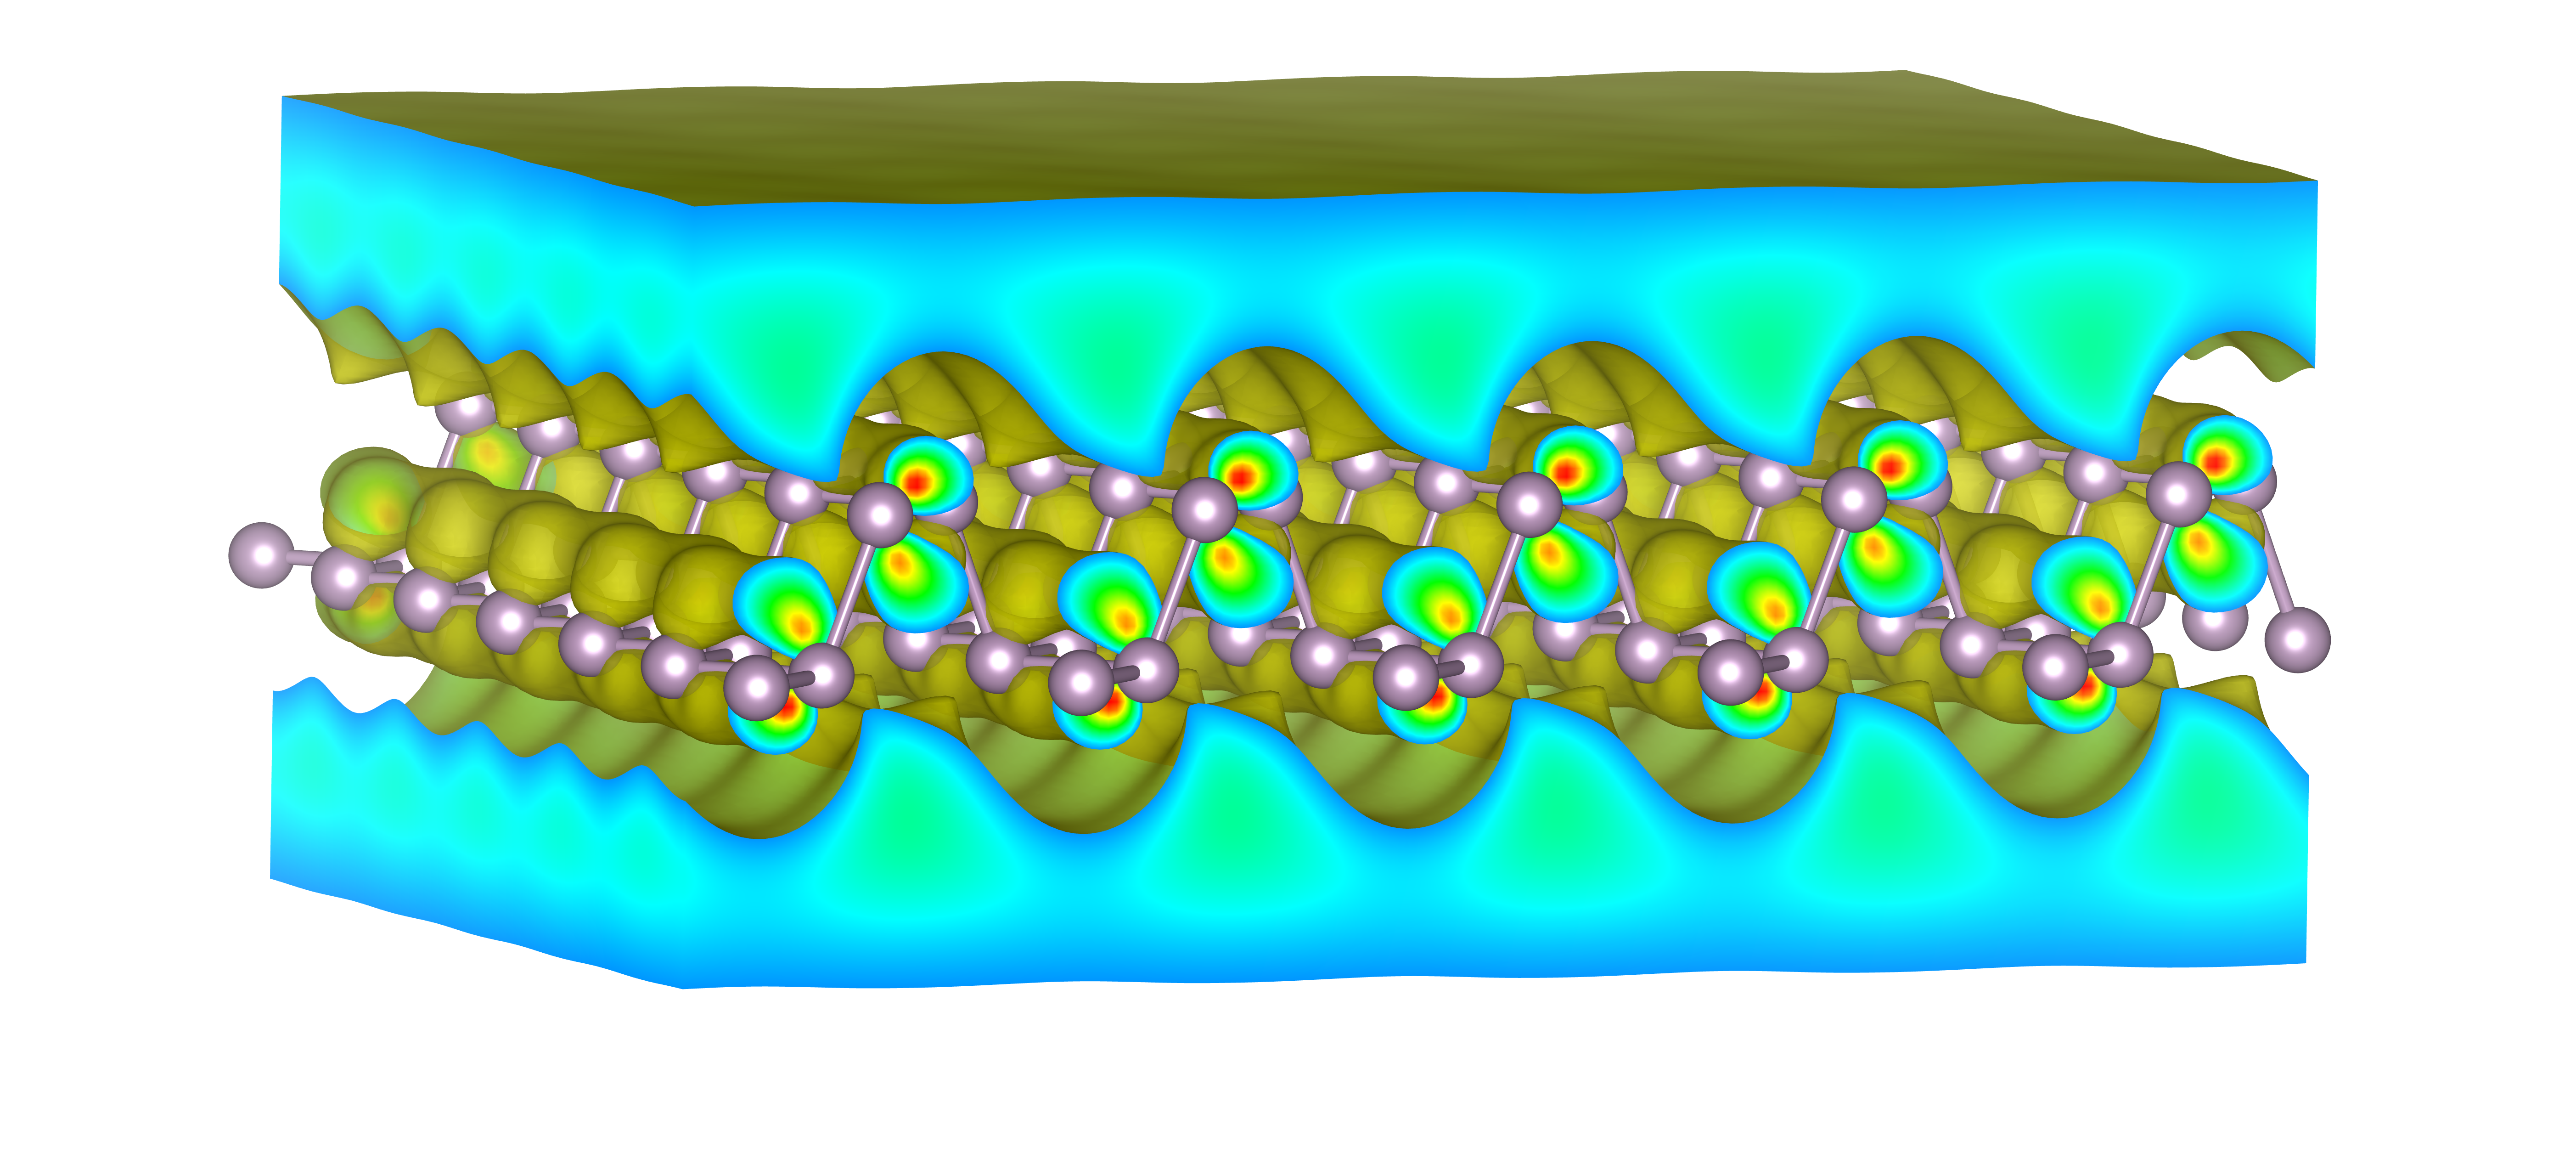
\includegraphics[width=\linewidth,angle=90]{figs/phos_gamma_cbm.png}
\end{figure}

\end{center}

\end{minipage}%
\hfill
\begin{minipage}[t]{0.33\textwidth}

\begin{center}
{\bf How?}
\begin{itemize}
  \item Q. Monte Carlo
\end{itemize}
\begin{figure}[h]
  \centering
  \includegraphics[width=0.7\linewidth]{figs/mc.png}
\end{figure}
\begin{itemize}
  \item $[$\texttt{CASINO} code$]$
\end{itemize}
\end{center}

\end{minipage}%
\hfill
\begin{minipage}[t]{0.33\textwidth}

\begin{center}
{\bf Why?}
\begin{itemize}
  \item Tech. {\tiny (Lopez-Sanchez {\it et al.}, Nat. Nano {\bf 8},
  (2013).)}
\end{itemize}
\begin{figure}[h]
  \centering
  \includegraphics[width=\linewidth]{figs/mos2.pdf}
\end{figure}
\begin{itemize}
  \item Methods.
\end{itemize}


\end{center}

\end{minipage}%

\btVFill

\centering
Ryan Hunt | \texttt{ryan.hunt@postgrad.manchester.ac.uk}

\end{frame}

\end{document}
